\subsection{X線回折パターン}
図\ref{fig:fig6}に、メソMD計算結果から求めたX線回折パターンを示す。
この図には、モデル1とモデル2両方の結果が示されている。
グラフの横軸はX線の回折角$2\theta$[deg]を、縦軸はX線強度$I$を示している。
各々のグラフには、7つのことなる圧縮段階におけるXRDパターンが示されており、
それぞれ図中に示した乾燥密度と間隙率のモデルに関するものである。
これらの結果には、圧縮の進行、すなわち、乾燥密度の増加にともない次第に強い
回折ピークが$2\theta=$6度付近に現れる様子が現れている。
これは、二層膨潤状態にある粘土の層間距離に対応し、実験でも観測されている
結果である。一方、回折ピークの鋭さは、組織構造の周期性を反映しており、
鋭いピークであるほど、積層数が多いことを意味する。
この点からモデル1とモデル2の回折パターンを比較すると、
モデル2のピークはモデル1に比べて鋭く、積層構造がより発達していることが分かる。
また、モデル1、モデル2の結果とも、乾燥密度が小さく、非常に緩く粘土が堆積
した状態でも、$2\theta=$5度付近にピークが現れており、圧縮の速い段階で
積層構造が現れ、平均的な層間距離が次第に詰まってはくるものの、積層数自体は
あまり大きくならないことが分かる。
%--------------------
\begin{figure}[h]
	\begin{center}
	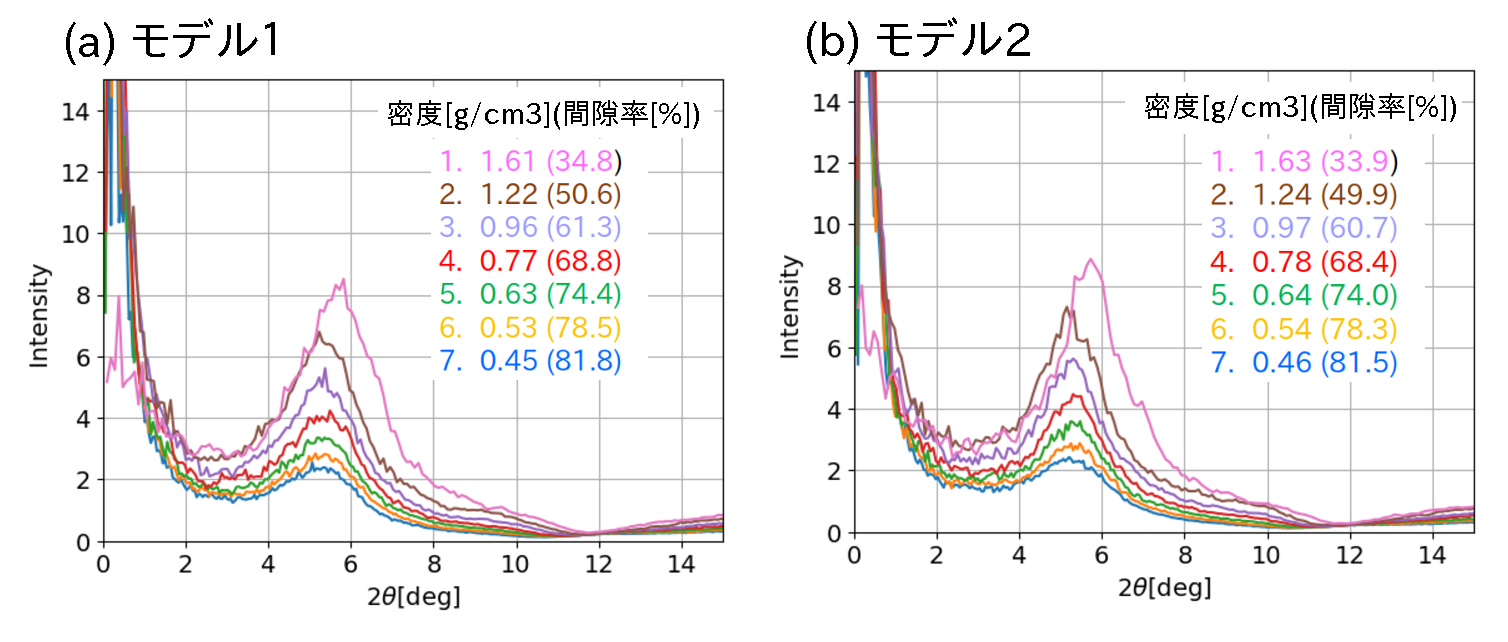
\includegraphics[width=1.0\linewidth]{Figs/fig6.eps} 
	\end{center}
	\caption{
		メソMDシミュレーションの結果から求めたX線回折パターン.
	} 
	\label{fig:fig6}
\end{figure}
%--------------------
\subsection{動径分布関数}
動径分布関数(RDF)の計算結果を図\ref{fig:fig7}に示す。
RDFについても、モデル1と2の両方に対する結果それぞれで、
7つの異なる密度の組織構造モデルに対して評価したRDFをプロットしている。
RDFのピークは、横軸で示された動径距離において、相対的に多数の
粗視化粒子が存在していることを示している。
ここに示した全てのRDFは複数のピークを示しており、ピーク位置にあたる
動径距離は概ね1.5nmとなっている。これは、二層膨潤状態における粘土層間距離に
一致しており、組織構造中に見出される粘土分子の積層状態が適切に
評価されていることを示している。
乾燥密度によるRDFの変化を見ると、RDFの値は乾燥密度の減少に応じて増加の傾向を
示すものの、グラフの形状はあまり変化しないことが分かる。
これは、圧縮の初期の段階で形成された積層構造が維持され、その後大きく発達
しないことを意味する。一方、モデル1とモデル2の結果を比較すると、
モデル1で明確なピークが3つであるのに対し、モデル2では5つ程度のピークが
見られる。これは、モデル1と2の組織構造の示す平均的な積層数がそれぞれ4層と6層である
ことを意味し、実験で取得したX線回折ピークの半値幅から推定される結果に近い値となっている。
これら、積層数と積層構造の形成時期に関する傾向は、XRDパターンから読み取ることが
できる傾向と整合している。
理論的には、RDFとXRDパターンは相互に変換可能であるため、両者の解釈はそもそも
一致すべきものである。ただし、本研究では、XRDパターンとRDFは異なる仮定の元、全く別の
方法で評価したものであることから、両者の結果から読み取れる情報が整合的であることは、
これらの分布関数の評価方法が妥当であったことを裏付けている。
%--------------------
\begin{figure}[h]
	\begin{center}
	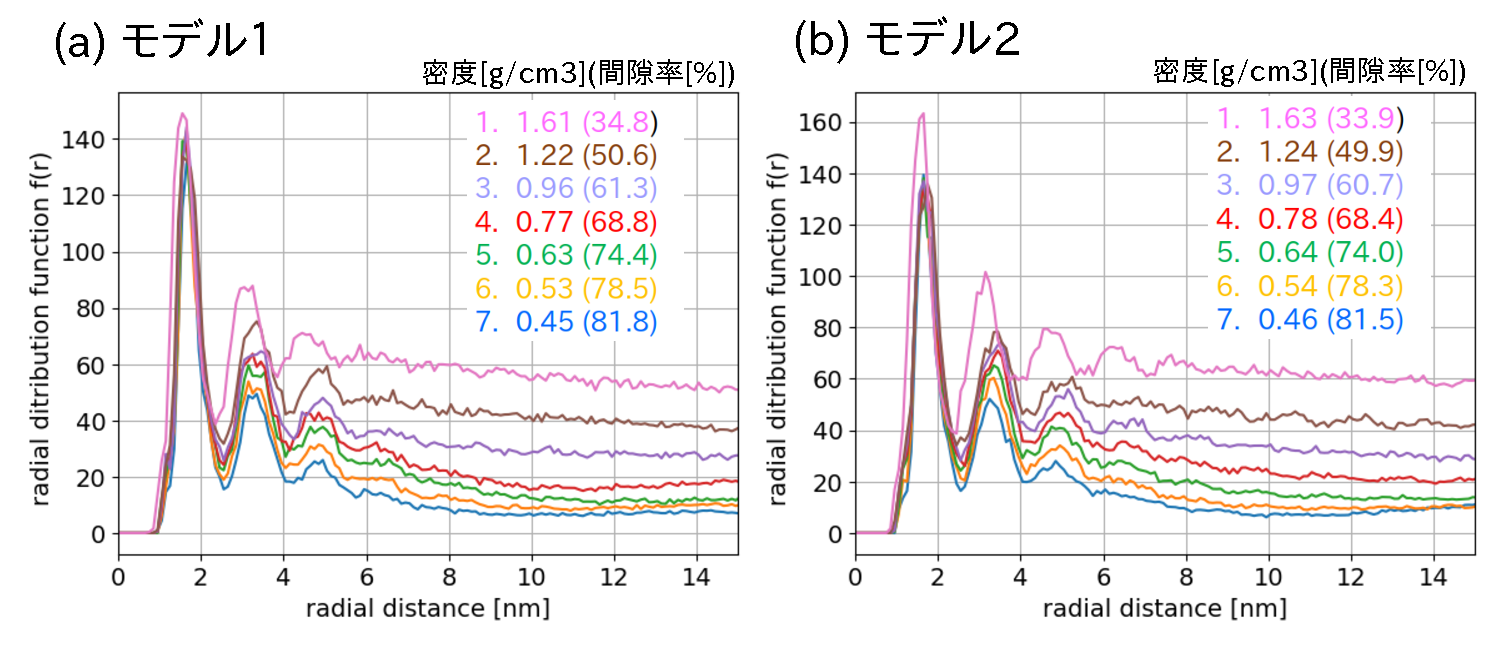
\includegraphics[width=1.0\linewidth]{Figs/fig7.eps} 
	\end{center}
	\caption{
		メソMDシミュレーションの結果から求めた動径分布関数.
	} 
	\label{fig:fig7}
\end{figure}
%--------------------
\subsection{数密度}
\subsubsection{確率密度関数}
局所密度を与える式(\ref{eqn:rhox_gen})において、$m_i=1$と置けば、
$\rho(\fat{x})$の値は粗視か粒子の数密度と一致する。
図\ref{fig:fig8}は,このことを利用して粒子の数密度を求め、
得られた数密度のヒストグラムを正規化し、確率密度分布として
示したものである。ここでも、モデル1と2、それぞれ7つの異なる乾燥密度に
に対する結果を示している。
乾燥密度が低いとき、密度がゼロ付近で大きな確率をとっている。
これは、空隙部分が広い範囲を占めていることの現れで、乾燥密度の増加に伴い
最終的には消失する。それと入れ替わるように、数密度0.6ふきんに顕著なピークが
現れる。ただし、緩やかなピークは、圧縮過程の初期の段階から、0.6付近に存在し、
これは、早い段階で粘土分子が凝集することを反映したものである。
なお、モデル1と2の結果を比較すると、モデル2のピークがより鋭いことが分かる。
これは、モデル2は粒径分布が広く、様々な粒径が混在することから、一定サイズの
ユニットセルを均等に埋めるようにパッキングされやすいことを示す、妥当な
結果であると言える。
%--------------------
\begin{figure}[h]
	\begin{center}
	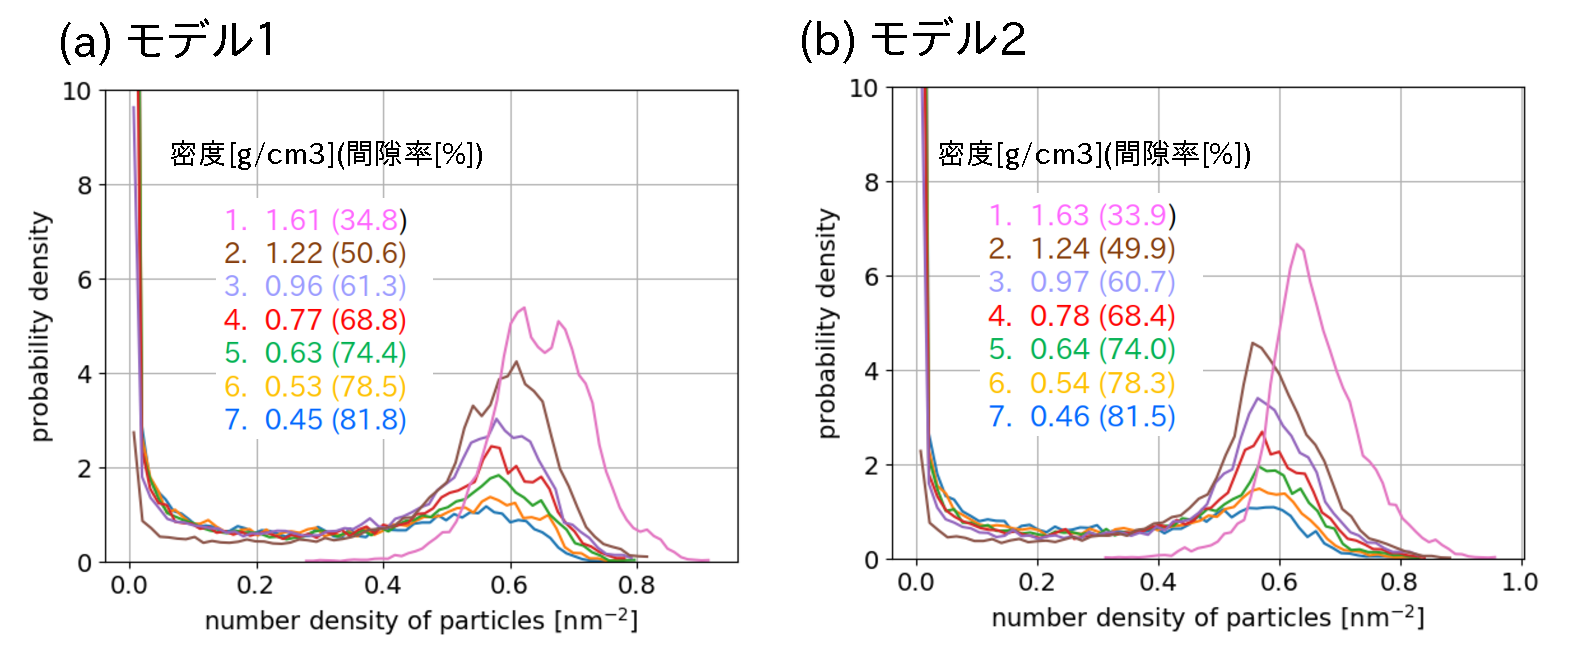
\includegraphics[width=1.0\linewidth]{Figs/fig8.eps} 
	\end{center}
	\caption{
		メソMDシミュレーションの結果から求めた数密度の確率確率密度分布.
	} 
	\label{fig:fig8}
\end{figure}
%--------------------
\subsubsection{空間分布の推移}
圧縮凝集過程における粒子数密度の推移を、図\ref{fig:fig10}と図\ref{fig:fig11}に
示す。これらは粒子数密度の空間分布を、6つの時刻におけるスナップショットとして
示したものである。数密度が小さな領域は青で、大きな部分は赤で示されており、
ごく初期の段階から、0.8程度の数密度を持つ箇所が現れ、これは、粘土が早々に積層構造
を作ることを示している。この結果からも、圧縮の途中段階で、積層構造があまり大きく
発達しないことが分かる。なお、モデル1と2に対する結果において、 例えば図\ref{fig:fig11}の(a)
と(d)を比較すると、モデル2の方がやや大きな空洞が残されている
ように見えるが、その他の点では2つのモデルで明確な違いは認められない。
ただし、ここに示した結果は、粘土層間の微細な間隙(ナノ間隙)と層外の比較的大きな
間隙(メソ間隙)の分布を用意に定量化できることを示している。スケールの異なる間隙では、
物質輸送挙動が異なることから、マクロスケールでの物質輸送解析を行う際、
空隙のサイズと連結性のモデルを与える必要があり、ここで示した密度分布に基づく
間隙の区分はそのようなモデル化作業において役立つと考えられる。
%--------------------
\begin{figure}[h]
	\begin{center}
	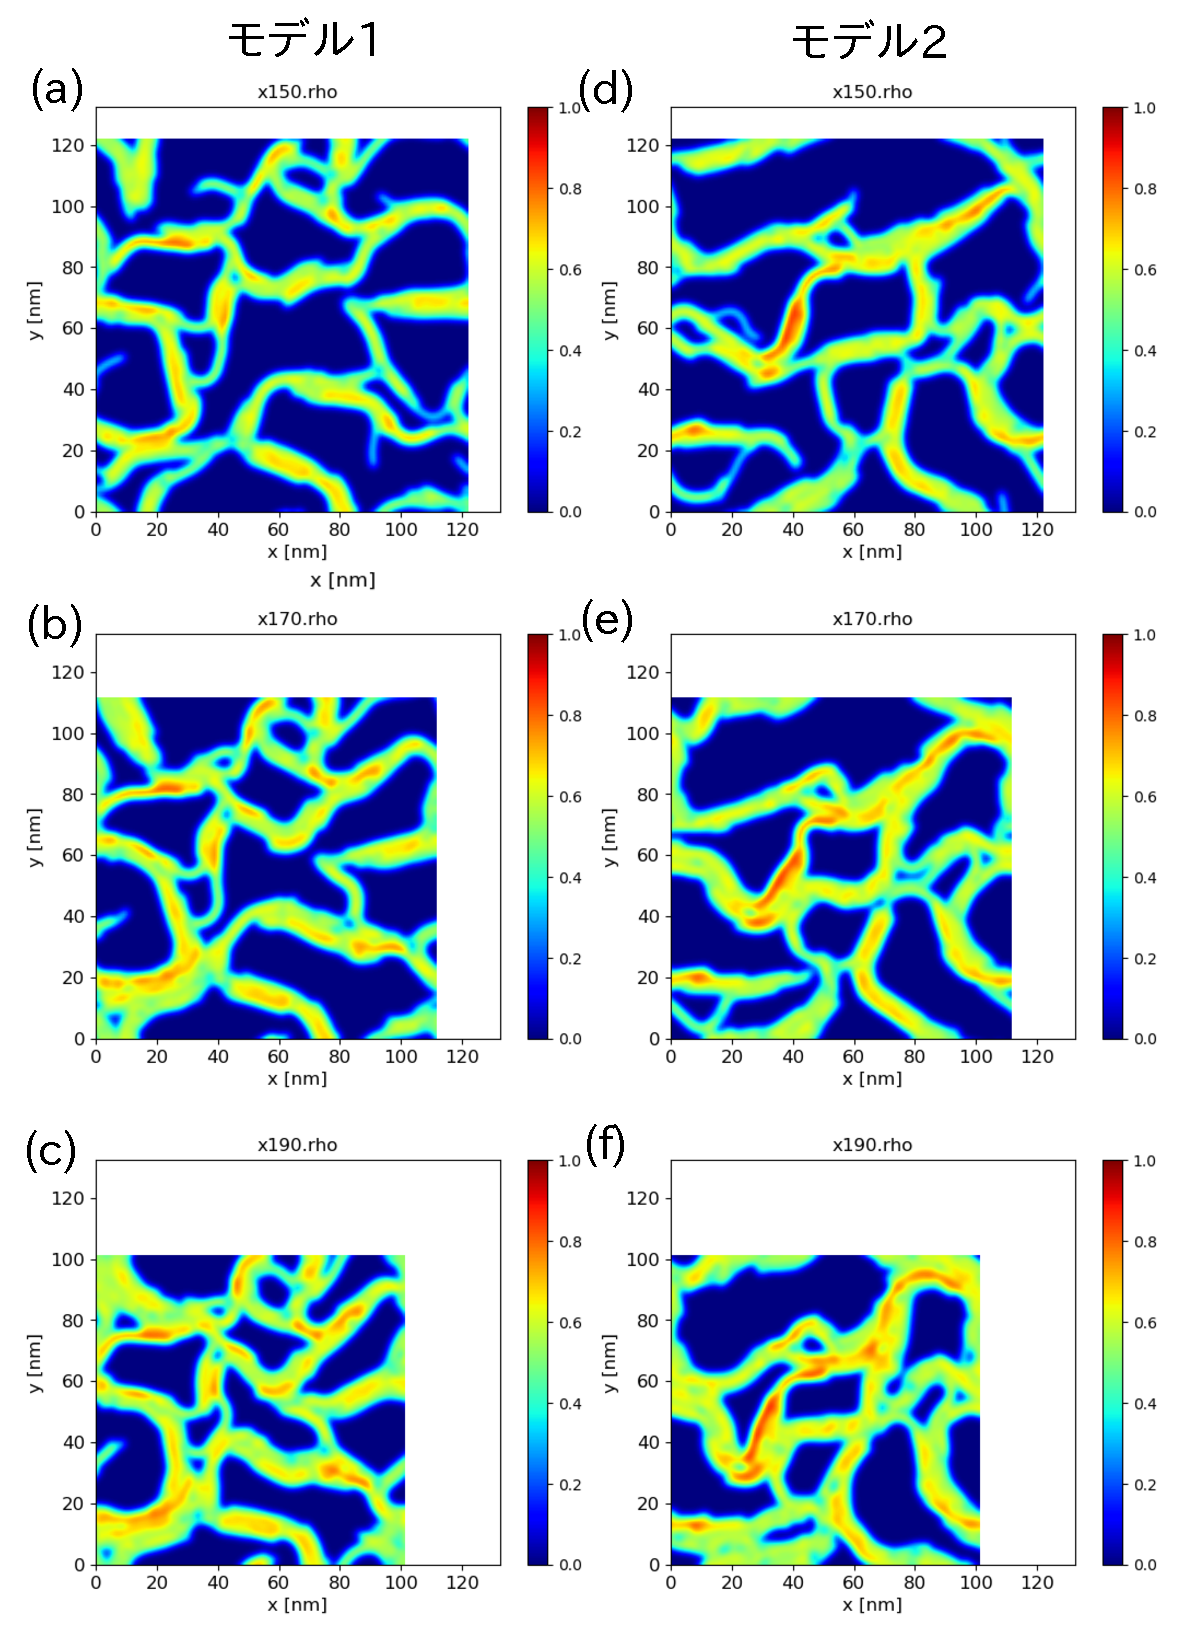
\includegraphics[width=1.0\linewidth]{Figs/fig10.eps} 
	\end{center}
	\caption{
		粒子数密度の空間分布(圧縮凝集過程の途中段階での状況を示すスナップショット).
	} 
	\label{fig:fig10}
\end{figure}
%--------------------
%--------------------
\begin{figure}[h]
	\begin{center}
	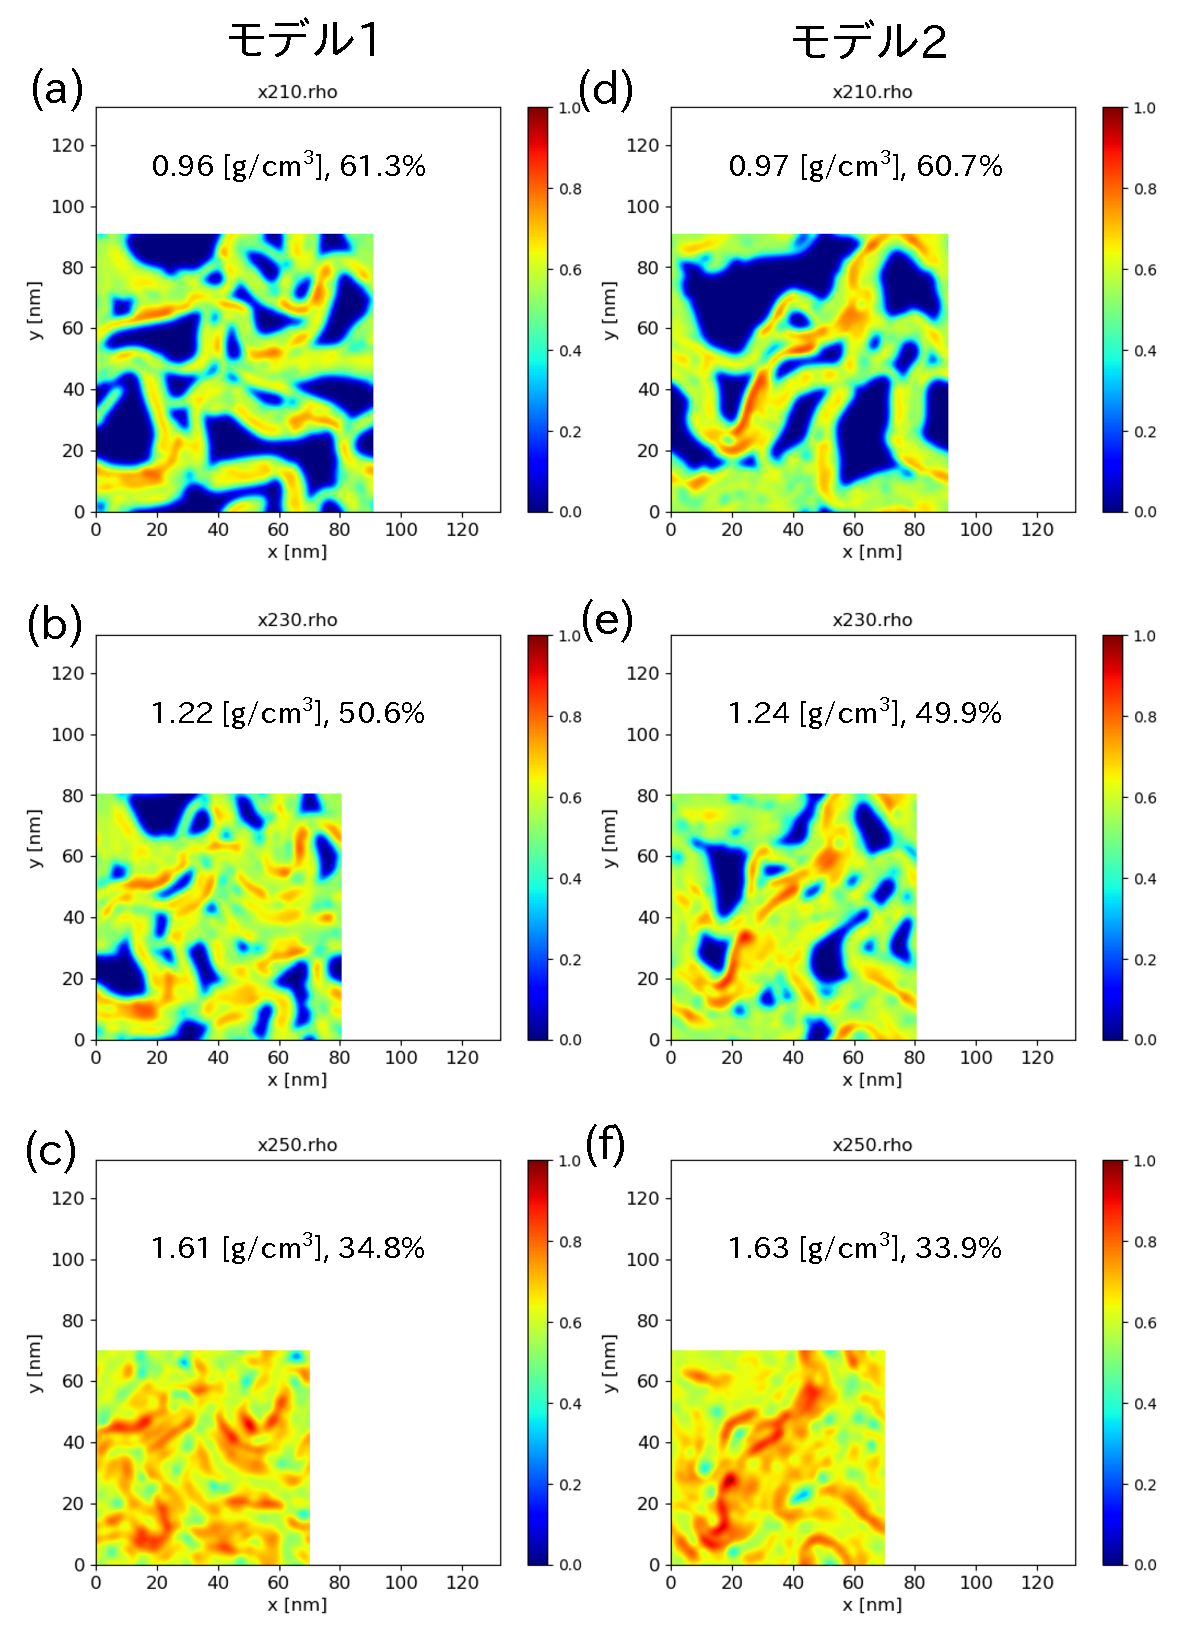
\includegraphics[width=1.0\linewidth]{Figs/fig11.eps} 
	\end{center}
	\caption{
		粒子数密度の空間分布(圧縮凝集過程の最終段階の状況を示すスナップショット).
	} 
	\label{fig:fig11}
\end{figure}
%--------------------
\subsection{粒子の配向性}
最後に、粗視化粒子の配向性について調べた結果を図\ref{fig:fig9}に示す。
このグラフは、ユニットセル中の全粗視か粒子の方向を調べ、
粒子方向$\alpha$[deg]の確率密度分布を求めた結果で、
7つの異なる乾燥密度における粒子の配向状態を示している。
モデル1と2に対する結果を比較すると、モデル1の方がやや強く配向
している様子が示されている。モデル1はおよそ$\alpha=$100度の方向に配向
しており、その傾向が圧縮の進行過程で持続している。このことは、
モデル1では、積層した粘土分子群はモデル2に比べて方向を変化させにくい
ことを示唆している。こういった挙動は、拡散係数等の物性値に異方性に
反映されることが予想されるため、明確な配向性が結果的に生じない場合においても、
組織構造解析の一貫として実施する価値のあることと思われる。
%--------------------
\begin{figure}[h]
	\begin{center}
	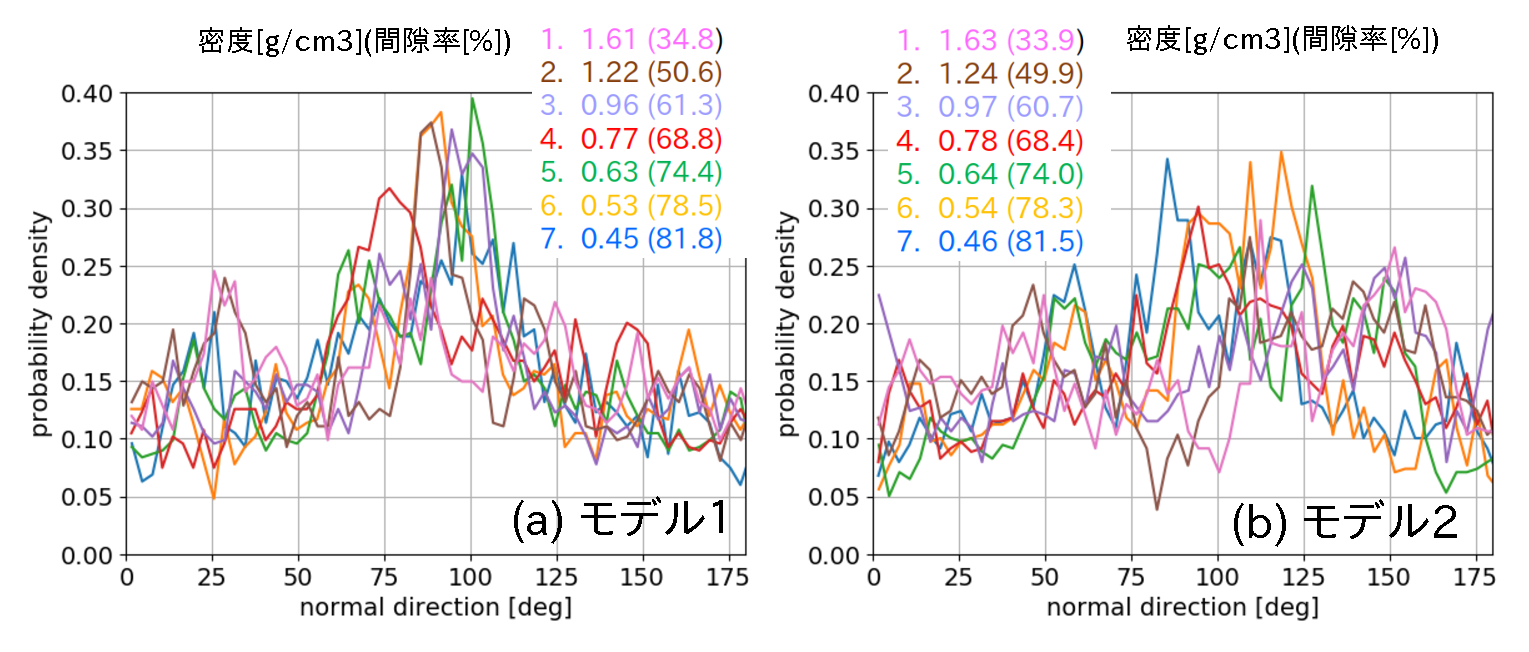
\includegraphics[width=1.0\linewidth]{Figs/fig9.eps} 
	\end{center}
	\caption{
		メソMDシミュレーションの結果から求めた粒子方向の確率密度分布.
	} 
	\label{fig:fig9}
\end{figure}
%--------------------
